\documentclass[a4paper, 6pt, landscape]{scrartcl}
\usepackage[german]{babel}
\usepackage[utf8]{inputenc}
\usepackage{multicol}
\usepackage{geometry}
\usepackage{graphicx}
\usepackage{wrapfig}
\usepackage{enumitem}
\usepackage{fancyhdr}
\usepackage{index}
\usepackage{sectsty}
\usepackage{mwe}
\usepackage{comment}
\usepackage{lipsum}
\usepackage{titlesec}
\usepackage[dvipsnames]{xcolor}
\usepackage{amsmath}
\usepackage{amssymb}


%Define Math Commands:
\newcommand*{\field}[1]{\mathbb{#1}}%
\newcommand{\Mod}[1]{\ (\mathrm{mod}\ #1)}

%Image Folder:
\graphicspath{{../img/}}

%format
\geometry{top=0.4cm,left=0.5cm,right=0.5cm,bottom=0.4cm}
\setlist{topsep=0pt, leftmargin=5mm, nolistsep}

% Code Snippets
\usepackage{courier} %% Sets font for listing as Courier.
\usepackage{listings}

\definecolor{javared}{rgb}{0.6,0,0} % for strings
\definecolor{sectionColor}{HTML}{7cbad4}
\definecolor{subSectionColor}{HTML}{c7e5b6}
\definecolor{subSubSectionColor}{HTML}{ffeca9}
\definecolor{royalBlue}{HTML}{4A1FBF}
\definecolor{midnightBlue}{HTML}{191970}
\definecolor{codeBackground}{RGB}{245,245,245}
\definecolor{gray}{rgb}{0.5,0.5,0.5}
\definecolor{lightgray}{rgb}{.9,.9,.9}
\definecolor{darkGreen}{RGB}{0,150,0}
\definecolor{DarkPurple}{rgb}{0.4, 0.1, 0.4}

\lstset{
frame=none,
captionpos=b,
escapeinside={*'}{'*},
language=Java,
tabsize=2,
commentstyle=\it,
stringstyle=\mdseries\rmfamily,
showspaces=false,
keywordstyle=\bfseries\color{RoyalBlue},
backgroundcolor=\color{lightgray},
columns=flexible,
basicstyle=\small\ttfamily,
showstringspaces=false,
morecomment=[l]\%,
aboveskip = 0.2em,
belowskip = 0.2em
}




% Define Section Format
\titleformat{name=\section}[block]{\sffamily\small}{}{0pt}{\colorsection}
\titlespacing*{\section}{0pt}{0pt}{0pt}
\newcommand{\colorsection}[1]{%
\colorbox{sectionColor!80}{\parbox{0.98\linewidth}{\vspace{-1pt}\color{black}\ #1 \vspace{-2pt}}}}

% Define Subsection Format
\titleformat{name=\subsection}[block]{\sffamily\small}{}{0pt}{\colorsubsection}
\titlespacing*{\subsection}{0pt}{0pt}{0pt}
\newcommand{\colorsubsection}[1]{%
\colorbox{subSectionColor!80}{\parbox{0.98\linewidth}{\vspace{-1pt}\color{black}\ #1 \vspace{-2pt}}}}

% Define SubSubsection Format
\titleformat{name=\subsubsection}[block]{\sffamily\small}{}{0pt}{\colorsubsubsection}
\titlespacing*{\subsubsection}{0pt}{0pt}{0pt}
\newcommand{\colorsubsubsection}[1]{%
\colorbox{subSubSectionColor!60}{\parbox{0.98\linewidth}{\vspace{-1pt}\color{black}\ #1 \vspace{-2pt}}}}


% -----------------------------------------------------------------------
\begin{document}
    %	\pagecolor{p}
    %	\color{t}
    \setlength{\columnseprule}{0.4pt}
    \footnotesize
    \begin{multicols*}{4}

        %! Author = Philipp Emmenegger
%! Date = 10/06/2021

\section{Multithreading Grundlagen}
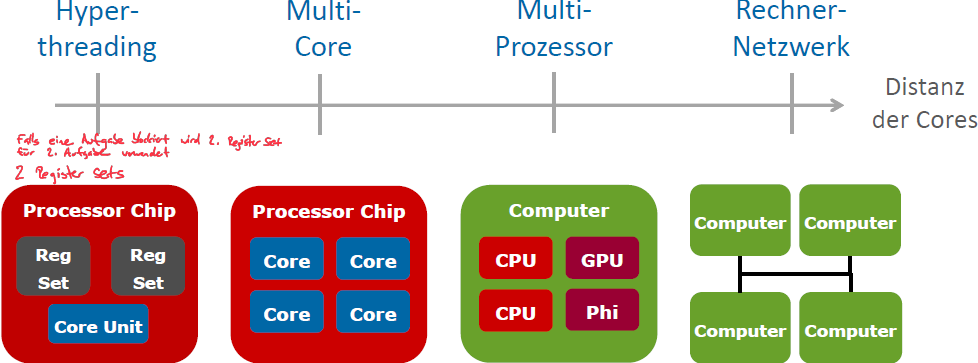
\includegraphics[width=\linewidth]{img/stufen.png}
\textbf{Parallelität:} Aufteilung in Teilabläufe, laufen gleichzeitig auf mehreren Prozessoren.
\textbf{Nebenläufigkeit:} Gleichzeitig oder verzahnt ausführbare Abläufe, greifen au gemeinsame Ressourcen zu.
\textbf{Prozess:} Parallel laufende Programm-Instanz im System. Eigener Adressraum.
\textbf{Thread:} Parallele Ablaufsequenz innerhalb eines Programms. Teilen gleichen Adressraum.

\subsection{Thread-Implementationen}
\textbf{User-Level Threads:} Im Prozess implementiert.
Keine echte Parallelität durch mehrere Prozessoren.
\textbf{Kernel-Level Threads:} Im Kernel implementiert (Multi-Core Ausnutzung).
Kontextwechsel vom Prozess per SW-Interrupt.
\textbf{Thread Scheduling:} Processor Sharing - \#Threads \textgreater \#Prozessoren.

\subsection{Prozessor Multiplexing}
\textbf{Verzahnte Ausführung:} Instruktionen von mehreren Threads in Teilsequenzen. Illusion der Parallelität.
\textbf{Kontextwechsel:} \textit{Synchron} (Freiwillige abgabe), Thread wechselt zu wait. \textit{Asynchron:} (gezwungene Abgabe) Begrenzte Laufzeit für Threads.

\subsection{Multi-Tasking:}
\textbf{Kooperativ:} Threads initiieren Kontextwechsel synchron (freiwillig). Scheduler kann Thread nicht unterbrechen.
\textbf{Preemtiv:} Scheduler kann Thread mit Timer-Interrupt asynchron unterbrechen (Time-Sliced-Scheduling)(\textit{Standart heute}).
\textbf{Thread Zustände:} Ready, Waiting, Running.

\subsection{Multi-Thread Programmierung}
\subsubsection{JVM Thread Modell}
Java ist ein Single Process System. 
JVM ist ein Prozess im Bsys.
\textbf{Main-Thread} wird beim Aufstarten der JVM anhand \textit{main()} Methode erzeugt.
JVM läuft, solange Threads laufen (Ausnahme Daemon Threads).
\begin{lstlisting}
var myThread = new Thread(() -> { /* ... */ });
myThread.start();
\end{lstlisting}
Thread wird erst bei \textit{start()} erzeugt. Führt \textit{run()}-Methode des Runnable Interface aus.
Thread endet beim Verlassen von \textit{run()}.\\
\textbf{Nicht-Determinismus:} Threads laufen ohne Vorkehrungen beliebig verzahnt oder parallel.
\subsubsection{Explizite Runnable-Implementation:}
\begin{lstlisting}
class SimpleLogic implements Runnable {
    @Override
    public void run() { /* ... */ }
}
var myThread = new Thread(new SimpleLogic()).start();
\end{lstlisting}

\subsubsection{Sub-Klasse von Thread}
\begin{lstlisting}
class SimpleThread extends Thread {
    @Override 
    public void run() { /* ... */ }
}
var myThread = new SimpleThread().start();
\end{lstlisting}

\subsubsection{Thread Join}
Warten auf Beendigung eines Threads. \textit{t2.join()} blockiert, solange t2 läuft.

\subsubsection{Thread Passivierung}
\textbf{Thraed.sleep(ms):} Laufender Thread geht in Wartezustand, dann ready.
\textbf{Thread.yield():} Gibt Prozesor frei, direkt ready.

    \end{multicols*}
\end{document}

























